\section{Příklady výstupu}

Vzhled výsledku se liší podle zvoleného vyhledávacího algoritmu. Pro oba dva algoritmy se zobrazí název skladby, autor, metrika algoritmu (délka nejdelší podsekvence pro LCS, vzdálenost pro DTW), pozice segmentu v skladbě a výpis melodie segmentu. U výpisu melodie je tlačítko pro její přehrání.

Pro LCS se navíc ve výpisu melodie segmentu zvýrazní zeleně noty, které patří do nalezené největší společné podsekvence.

Pro DTW se zobrazí graf porovnávající dotaz a segment. Zobrazuje se v něm navíc mapování členů sekvencí. Grafy se generují v backendu při zpracování dotazu pomocí knihovny \textit{Matplotlib} a po jejich vygenerování jsou podávány frontendu jako obrázky.

\begin{figure}[!ht]
    \centering
    \caption{Vstupní melodie}
    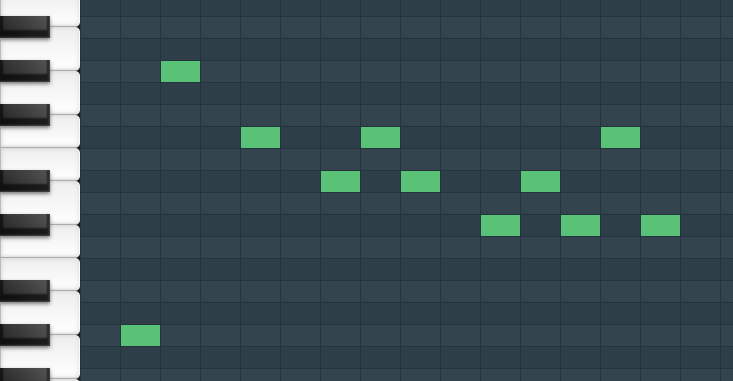
\includegraphics[width=\textwidth]{images/input_melody.png}
\end{figure}

\begin{figure}[!ht]
    \centering
    \caption{První dva nejlepší výsledky LCS}
    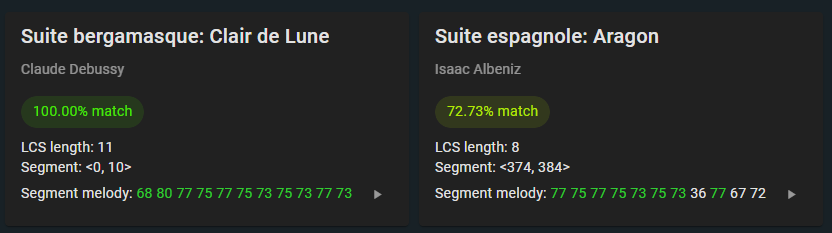
\includegraphics[width=\textwidth]{images/lcs_results.png}
\end{figure}

\pagebreak

\begin{figure}[!ht]
    \centering
    \caption{První dva nejlepší výsledky DTW}
    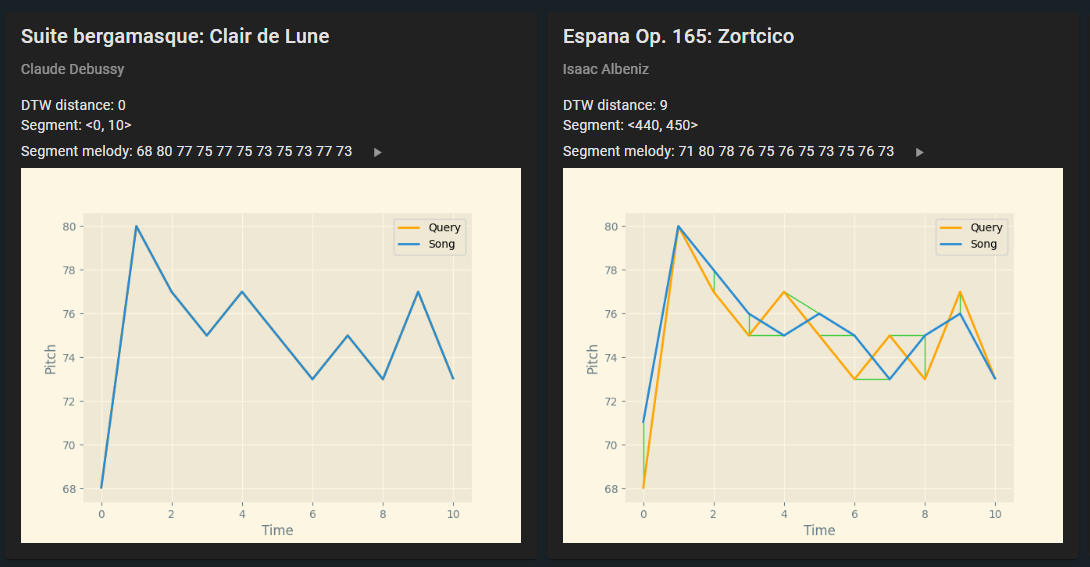
\includegraphics[width=\textwidth]{images/dtw_results.png}
\end{figure}

\begin{figure}[!ht]
    \centering
    \caption{Detail grafu DTW pro druhý výsledek}
    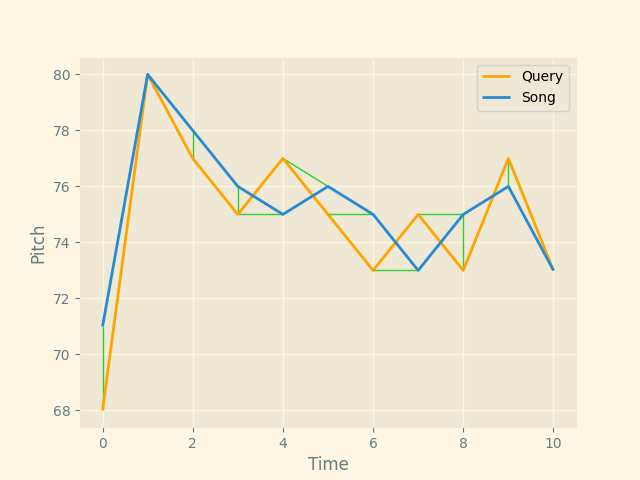
\includegraphics[width=\textwidth]{images/dtw_graph_example.png}
\end{figure}

\pagebreak